\chapter{Related Work}
\section{Supervised Learning for Fake News Detection\cite{Reis2019}}
Reis et al. use machine learning techniques on buzzfeed article related to US election. The evaluated algorithm are k-Nearest Neighbors, Na\"ive-Bayes, Random Forests, SVM with RBF kernel and XGBoost. \\

In order to feed this network they used a lot of hand-crafted features such as 
\begin{itemize}
	\item Language Features: bag-of-words, POS tagging and others for a total of 31 differents features,
	\item Lexial Features: amount of uniques words and their frenquencies, pronouns, etc,
	\item Pyschological Features\cite{Pennebaker2001}: build using Linguistic Inquiry and Word Count which is a specific dictionary build by a text mining software,
	\item Semantic Features: Toxic score from Google's API,
	\item Engagement: Number of comments within several time interval.
\end{itemize}

Many other features where also used, based on the source and social metadata. \\

Their results is shown at \textbf{Figure \ref{fig:chap1:reis}}.

\begin{figure}[h]
	\centering
	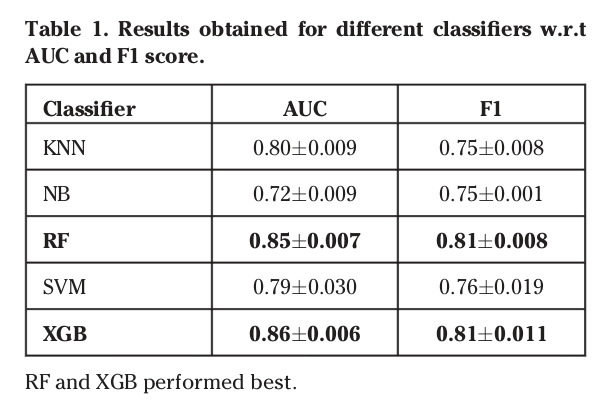
\includegraphics[width=0.5\textwidth]{images/chap1_bis/rev1.png}
	\caption{Results by Reis et al. }
	\label{fig:chap1:reis}
\end{figure}

They also shows that XGBoost is good for selecting texts that need to be hand verfied. This model is limited by the fact they do use metadata that are not always available. 

P\'erez-Rosas et al.\cite{Perez-Rosas2017} used almost the same set of features but used linear SVM as a model and worked on a different dataset.

\section{CSI: A Hybrid Deep Model for Fake News Detection}
Ruchansky et al.\cite{Ruchansky2017} used an hybrid network, merging news content features and metadata such as social engagement in a single network. To do so, they used an RNN for extracting temporal features of news content and a fully connected network in the case of social features. The results of the two network is then concatenated and use for final classification. \\

As textual features they used doc2vec\cite{Le2014}. \\

Network's architecture is shown at \textbf{Figure \ref{fig:chap1:Ruchansky}}.

\begin{figure}[h]
	\centering
	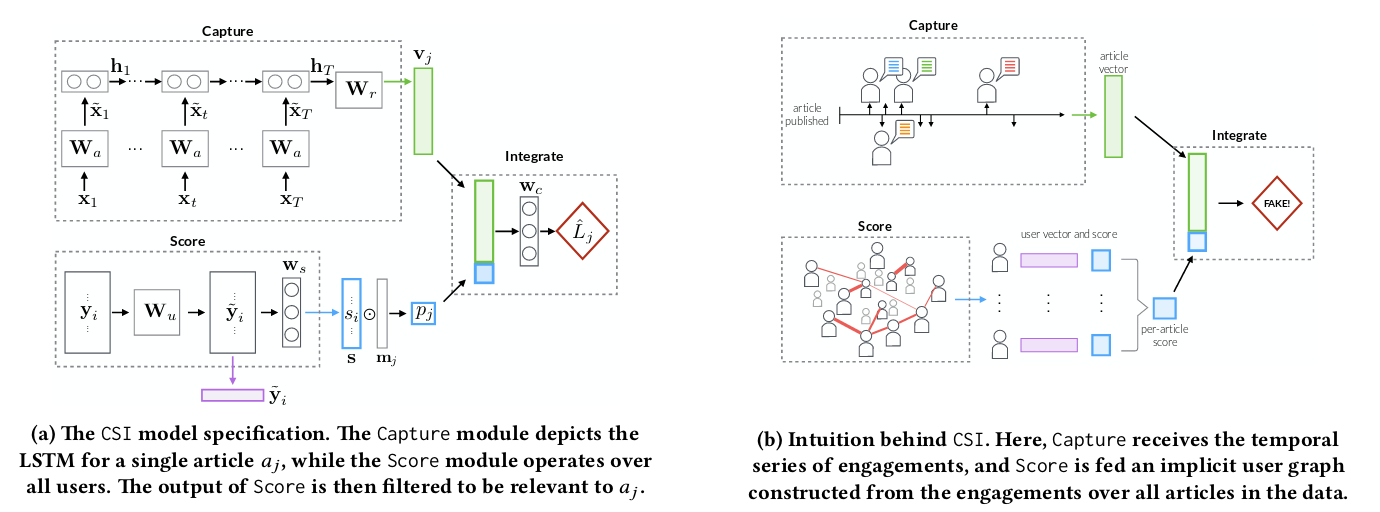
\includegraphics[width=\textwidth]{images/chap1_bis/rev2.png}
	\caption{CSI model}
	\label{fig:chap1:Ruchansky}
\end{figure}

They did test their model on two datasets, one from Twitter and the other one from Weibo, which a Chinese equivalant of Twitter. Compared to simpler models, CSI performs better, with $6\%$ improvement over simple GRU network (\textbf{Figure \ref{fig:chap1:Ruchansky2}}). 

\begin{figure}[h]
	\centering
	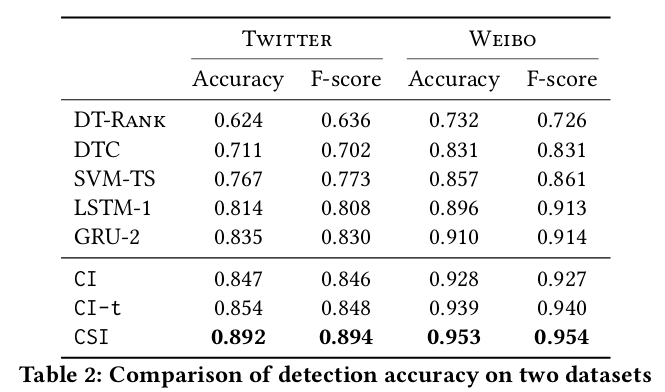
\includegraphics[width=0.5\textwidth]{images/chap1_bis/rev3.png}
	\caption{Results by Ruchansky et al. }
	\label{fig:chap1:Ruchansky2}
\end{figure}

\section{Some Like it Hoax: Automated Fake News Detection in Social Networks \cite{Tacchini2017}}
Here, Tacchini et al. focus on using social network features in order to improve the reliability of their detector. The dataset was collected using Facebook Graph API, collection pages from two mains categories: scientific news and conspiracy news. They used logistic regression and harmonic algorithm\cite{NIPS2011_4396} to classify news in categories hoax and non hoax. Harminoc Algorithm is a method that allows to transfer information across users who liked some common posts. \\

For the training they used cross-validation, dividing the dataset into $80\%$ for training and $20\%$ for testing and performing 5-fold cross-validation, reaching $99\%$ of accuracy in both cases. \\

In addition they used one-page out, using posts from a single page as test data or using half of the page as training and the other half as testing. This still lead to good results, harmonic algorithm outperforming logistic regression. Results are shown at \textbf{Figures \ref{fig:chap1:tacchini}} and \textbf{\ref{fig:chap1:tacchini2}}. \\


\begin{figure}[h]
	\centering
	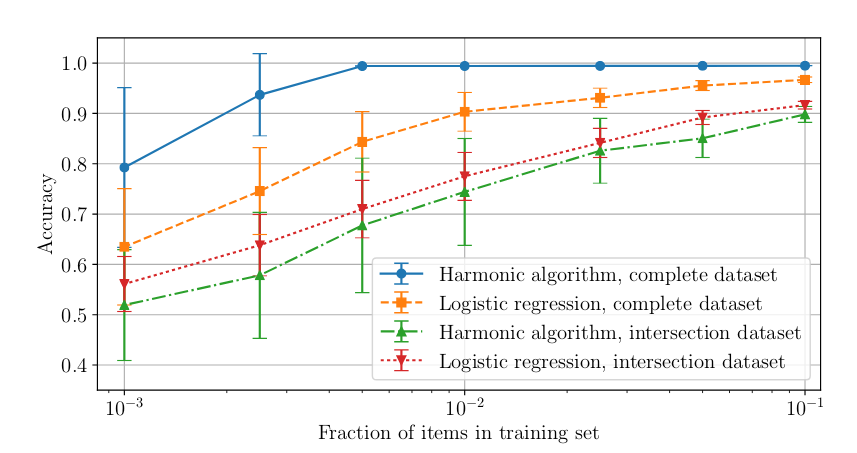
\includegraphics[width=0.7\textwidth]{images/chap1_bis/rev4.png}
	\caption{Results by tacchnini et al. }
	\label{fig:chap1:tacchini}
\end{figure}

\begin{figure}[h]
	\centering
	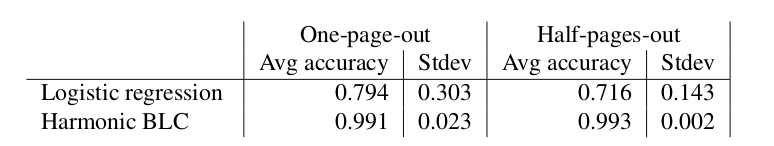
\includegraphics[width=0.7\textwidth]{images/chap1_bis/rev5.png}
	\caption{Results by tacchnini et al. }
	\label{fig:chap1:tacchini2}
\end{figure}